\documentclass[a4,abstract=on]{scrartcl}

\usepackage[utf8]{inputenc}
\usepackage[T1]{fontenc}
\usepackage{placeins}
\usepackage{graphicx}
\usepackage[hypcap]{caption}
\usepackage{algorithm}
\usepackage[noend]{algpseudocode}
\usepackage[hidelinks]{hyperref}
\usepackage[nochapters]{classicthesis} % nochapters, wenn du section als oberste ebene nimmst
\usepackage{array}
\PassOptionsToPackage{big}{titlesec}

\floatname{algorithm}{Algorithmus}
% Mathe
\usepackage{amsmath}
\usepackage{amssymb}


% Verlinkungen
\usepackage[ngerman]{varioref} % Siehe http://en.wikibooks.org/wiki/LaTeX/Labels_and_Cross-referencing#The_varioref_package
%\usepackage[hidelinks]{hyperref}

% Spracheinstellungen sowie Umlaute etc.
\usepackage[ngerman]{babel}
\usepackage{ngerman}

% Bilder
\usepackage{graphicx}

% Tabellen-Abstand
\renewcommand{\arraystretch}{1.5}

% Quellcode
\usepackage{listings}
\lstset{%
	breaklines=true,
	frame=single,
	keepspaces=true,
	numbers=left,
	numbersep=5pt,
	tabsize=2
}

% Literatur
\usepackage{bibgerm}
\usepackage{natbib}

% Lässt sections immer auf der ungeraden (rechten) Seite anfangen.
    \newcommand*\stdsection{}
    \let\stdsection\section
    \renewcommand*\section{%
    \clearpage\ifodd\value{page}\else\mbox{}\clearpage\fi
    \stdsection}

% neuer Typ von Tabellenspalte (so wie c, l, etc.). Ist zentriert mit fester Breite.
\newcolumntype{C}[1]{>{\centering\let\newline\\\arraybackslash\hspace{0pt}}m{#1}}

% \usepackage{setspace}
% \onehalfspacing
\title{Untersuchung verschiedener Kodierungen von speziellen Cardinality Constraints für SAT}
\date{~}

\begin{document}
	\maketitle
\thispagestyle{empty}
\begin{center}
\begin{Large}
Bachelorarbeit\\Universität Bremen\\Fachbereich $3$\\
~\\~\\
\textbf{Jil Tietjen}\\<jiltietj@informatik.uni-bremen.de>\\
~\\~\\
Erstgutachter: Prof. Dr. Rolf Drechsler\\
Zweitgutachter: Prof. Dr. Rüdiger Ehlers\\~\\
\mbox{Betreuung: Prof. Dr. Rolf Drechsler \&~Oliver Keszöcze}\\~\\~\\~\\~\\~\\~\\~\\
Bremen, $09$. Juni $2016$
\end{Large}
\end{center}
		
	\newpage
~\\
\textbf{Urheberrechtliche Erklärung}\\
Erklärung gem. § $10$ ($10$) Allgemeiner Teil der BPO vom $27$.$10$.$2010$
Hiermit versichere ich, dass ich meine Bachelorarbeit ohne fremde Hilfe angefertigt habe, und dass ich keine anderen als die von mir angegebenen Quellen und Hilfsmittel benutzt habe.\\
Alle Stellen, die wörtlich oder sinngemäß aus Veröffentlichungen entnommen sind, habe ich unter Angabe der Quellen als solche kenntlich gemacht.\\
Die Bachelorarbeit darf nach Abgabe nicht mehr verändert werden.\\
~\\~\\~\\
Bremen, den $09$.$06$.$2016$\\
~\\~\\~\\
Jil Tietjen
~\\~\\~\\~\\~\\~\\
Ich bin damit einverstanden, dass meine Abschlussarbeit im Universitätsarchiv für wissenschaftliche Zwecke von Dritten eingesehen werden darf.\\
~\\~\\~\\
Bremen, den $09$.$06$.$2016$\\
~\\~\\~\\
Jil Tietjen
\clearpage

	\tableofcontents
	\clearpage

\section{Einleitung}
\section{Grundlagen}
\section{Kodierungen}
In diesem Kapitel werden die unterschiedlichen Kodierungen beschrieben. Das Ziel ist es, dass die Cardinality Constraints über die Menge der Boolschen Variablen in eine Konjunktive Normalform (KNF) gebracht werden. %Innerhalb der KNF gibt es Einschränkungen, die verlangen, dass höchstens $r$ der Booleschen Variablen 1 sein kann. Rein in die Grundlagen
Das Cardinality Constraint ist nur erfüllt, wenn die Variablen unter der Berücksichtigung der Constraints mit $1$ belegt werden können. 

%Die einfachste Möglichkeit ein Cardinality Constraint zu kodieren basiert auf einem Bit-Addierer, in den alle Variablen nach und nach reingegeben werden. Das Ergebnis ist eine binäre Repräsentation der Integer und es wird durch die Boolschen Variablen bestimmt, das innerhalb des durch die Constraints vorgeschriebenen Bereichs ist. Ein Vorteil ist, dass die Größe der KNF nicht ausufert, aber dennoch müssen alle Variablen einen Wert haben, um diesen mit dem Constraint in SAT vergleichen zu können. 
%Evaluation Alle Kodierungen werden anhand des Damen-Problems auf ihre Praxistauglichkeit überprüft.

	\subsection{naiver Ansatz}

	\subsection{Kodierung nach Bailleux und Boufkhad}
Im folgenden wird die Kodierung aus  \cite[][]{bailleux} vorgetellt.
%Diese Kodierung ist, laut Bailleux, effizient mit Berücksichtigung der Unit Propagation, die in den meisten Sat-Solvern verwendet wird. Es werden O(n log (n)) Variablen und O($\text{n}^2$) Klauseln gefordert, die aus mindestens 3 Literalen bestehen. Bei dieser Kodierung ist das Besondere, dass es eine einstellige Darstellung von Integer-Variablen gibt, die nicht nur den Wert an sich repräsentieren, sondern auch einem Intervall zugeordnet werden kann. Zum Beispiel gilt die Variable c nur, wenn das Intervall der Variablen ($a + b$) c erfüllt. Dadurch erhält man eine KNF. Die Kodierung muss korrekt sein, wenn es eine wahre Zuordnung gibt die unter der Berücksichtigung der Constraints erfüllbar ist.

Bei dieser Kodierung können die Menge der Variablen (input, output und linking Variablen) als binärer Baum beschrieben werden.

%n erklären in den Grundlagen
Der Baum wird iterativ aufgebaut und beginnt mit einem Wurzelknoten, der mit 1 betitelt wird. Des Weiteren gibt es $n-1$ interne Knoten, sowie n Blätter, die von n bis $2n-1$ beschriftet werden. Die Kinder von Knoten k  für $1 \leq k \textless n$, sind die Knoten $2k$ und $2k +1$. Dies wird so lange wiederholt bis das letzte Blatt erreicht ist.
Jedem Knoten wird eine Menge von Variablen zugeordnet. Dabei wird jedem Blatt eine Eingangsvariable und dem Wurzelknoten eine Menge von Ausgangsvariablen zugerodnet. Nun wurd die Kodierung so aufgebaut, dass die Variablen eines inneren Knotens die Summe der Variablen seiner Kindsknoten repräsentieren. Daraus ergibt sich ein Wurzelknoten dessen Variablen mit r verglichen werden können.\\

Als nächster Schritt werden neue Variablen der Form $\text{b}_j^k$ gebildet, für die gilt, dass $1 \textless k \textless n$ und  $1 \leq j \leq t_k$ ist. $t_k$ ist dabei das Minimum von r und die Anzahl der Blätter unter dem Knoten k. Jedem inneren Knoten k wird die Menge der Variablen $\text{b}_j^k$ zugeordnet.\\
Mit den neuen Variablen können folgende Formeln gebildet werden:\\
\textbf{1. Formel:}\\
$ \neg \text{b}_i^{2k} \vee \neg \text{b}_j^{2k+1} \vee \neg \text{b}_{i+j}^{k}$ \\
für $0\leq i \leq \text{t}_{2k}$, $0\leq j \leq \text{t}_{2k+1}$, $1\leq i+j \leq \text{t}_{k}+1$, $1\textless k \textless n$\\
\textbf{2. Formel:}\\
$ \neg \text{b}_i^2 \vee \neg \text{b}_j^3$ für $0\leq i \leq \text{t}_2$, $0\leq j \leq \text{t}_3$, $i+j = r+1$\\

Dabei wird $\text{t}_k$ zu $1$ und $\text{b}_1^k = \text{x}_{k-n+1}$ für $n \leq k \textless 2n$. Dadurch können aus den Hilfsvariablen die entsprechenden Literale gebildet werden, die die KNF bilden.
Alle neu entstandenen Literale mit $\neg \text{b}_0^k$ und $\text{b}_{r+1}^k$ werden gestrichen. Dies hat keine weiteren Auswirkungen, da es nur triviale Variablen sind, die gestrichen werden dürfen.



\subsubsection{Beispiel für die Kodierung}
Für das Beispiel ist $n=4$ und $r =1$. Der binäre Baum hat $4-1 = 3$ interne Knoten, sowie 4 Blätter, die beschriftet sind mit 4 bis $2*4-1=7$. Die Kinder von Knoten $1$  für $1 \leq 1 \textless 4$, sind die Knoten 2 und $2*1 +1=3$. Daraus ergibt sich der binäre Baum, der in Abbildung \ref{fig:baum} zu sehen ist.

\begin{figure}[H]
\centering
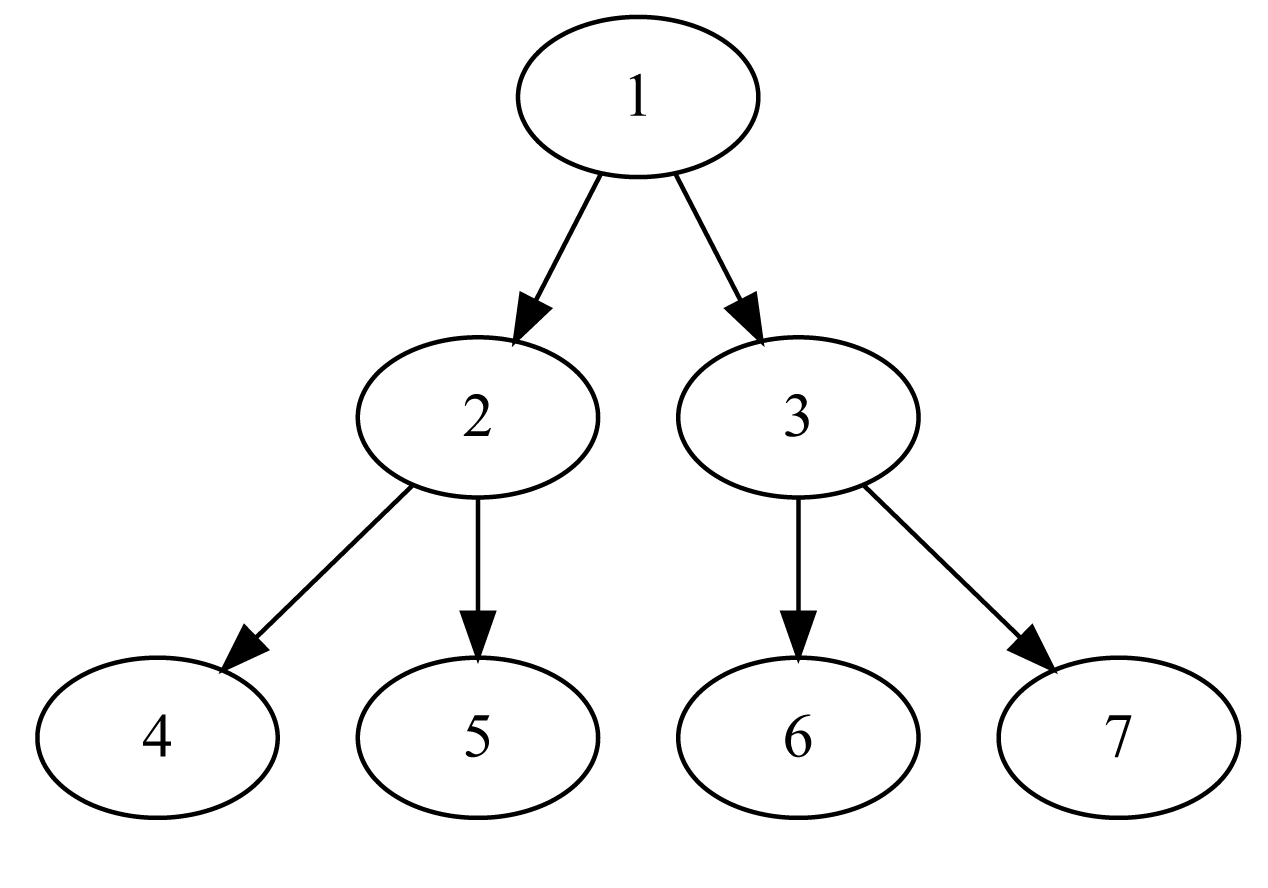
\includegraphics[width=6cm]{Bailleux_baum.png}
\caption{Binärer Baum nach Bailleux}
\label{fig:baum}
\end{figure}

$\text{t}_1$ hat nach oben genannter Formel 4 Blätter, $\text{t}_2$ und $\text{t}_3$ jeweils 2 und $\text{t}_4$ bis $\text{t}_7$ keine Blätter

Dadurch ergeben sich für das Beispiel von $n=4$ folgende Variablen:\\
\textbf{Formel 1:}\\
$k=2$ oder $k=3$, weil $1 \textless k \textless n$.\\
$j=0$ oder $j=1$, weil $1 \leq j \leq \text{t}_k$. $\text{t}_k = 1$, da es das Minimum von r ist.\\
$i=0$ oder $i=1$, weil $1\leq i+j \leq \text{t}_{k}+1$.\\
Somit wird in die folgenden Formeln $(i,j) = (1,0) \vee (0,1) \vee (1,1)$ eingesetzt.\\
\textbf{k = 2:}\\
$\neg \text{b}_1^4 \vee \neg \text{b}_0^5 \vee \text{b}_1^2$\\
$\neg \text{b}_0^4 \vee \neg \text{b}_1^5 \vee \text{b}_1^2$\\
$\neg \text{b}_1^4 \vee \neg \text{b}_1^5 \vee \text{b}_2^2$\\
\textbf{k = 3:}\\
$\neg \text{b}_1^6 \vee \neg \text{b}_0^7 \vee \text{b}_1^3$\\
$\neg \text{b}_0^6 \vee \neg \text{b}_1^7 \vee \text{b}_1^3$\\
$\neg \text{b}_1^6 \vee \neg \text{b}_1^7 \vee \text{b}_2^3$\\

Da alle der Form $\neg \text{b}_0^k$ und $\text{b}_{r+1}^k$  gestrichen werden, bleiben nur noch diese Variablen übrig:\\
\textbf{k = 2:}\\
$\neg \text{b}_1^4  \vee \text{b}_1^2$\\
$\neg \text{b}_1^5 \vee \text{b}_1^2$\\
$\neg \text{b}_1^4 \vee \neg \text{b}_1^5$\\
\textbf{k = 3:}\\
$\neg \text{b}_1^6 \vee \text{b}_1^3$\\
$\neg \text{b}_1^7 \vee \text{b}_1^3$\\
$\neg \text{b}_1^6 \vee \neg \text{b}_1^7 $\\

 Bildung der Literale:\\
$\neg \text{b}_1^4 = \neg \text{x}_1$, weil $\text{x}_{4-4+1}=\text{x}_1$ ist.\\
 Und alle anderen werden zu:\\
$ \neg \text{x}_1 \vee \neg \text{x}_3$\\
$\neg \text{x}_2 \vee \neg \text{x}_4$\\
$\neg \text{x}_2 \vee \neg \text{x}_3$\\
$\neg \text{x}_3 \vee \neg \text{x}_0$\\
$\neg \text{x}_4 \vee \neg \text{x}_0$\\
$\neg \text{x}_3 \vee \neg \text{x}_4$\\

\textbf{Formel 2:}\\
$i=0$, $i=1$ oder $i=2$, weil $0\leq i \leq \text{t}_2$ für $\text{t}_2 = 2$.\\
$j=0$, $j=1$ oder $j=2$, weil $0\leq j \leq \text{t}_3$ für $\text{t}_3=2$.\\
Somit wird in die folgenden Formeln $(i,j) = (1,1) \vee (0,2) \vee (2,0)$ eingesetzt, damit $i+j = r+1$ gilt.\\
$\neg \text{b}_1^2 \vee \neg \text{b}_1^3$\\
$\neg \text{b}_0^2 \vee \neg \text{b}_2^3$\\
$\neg \text{b}_2^2 \vee \neg \text{b}_0^3$\\

Alle trivialen Variablen werden gestrichen:\\
$\neg \text{b}_1^2 \vee \neg \text{b}_1^3$\\
$\neg \text{b}_2^3$\\
$\neg \text{b}_2^2$ \\

Daraus werden folgende Literale gebildet:\\
$\neg \text{x}_3 \vee \neg \text{x}_0$\\
$\neg \text{x}_0$\\
$\neg \text{x}_3$\\



%eigene Kodierung hervorheben am Ende
		

	\subsection{Kodierungen nach Sinz}
		\subsubsection{sequentiell}
		\subsubsection{parallel}

	\subsection{Kodierungen basierend auf Sorting Networks}
		\subsubsection{naiv}
		\subsubsection{Eén und Sörensson}

	\subsection{Entwickelte Kodierung auf Grundlage von Bailleux und Boufkhad}

\section{Umsetzung}
 Als Testproblem für die unterschiedlichen Kodierungen wird das n-Damen-Problem verwendet, da dieses Problem eine wichtige Rolle in der Informatik spielt und viele Constraints abgeleitet werden können. In jeder Reihe (vertikal, horizontal und diagonal) ist nur eine Dame erlaubt. Somit ergeben sich unterschiedliche Kombinationen, die für die Belegung der Literale nur erlaubt sind. Ziel ist es eine Belegung zu finden, die alle Bedingungen erfüllt.

\begin{figure}[H]
\centering
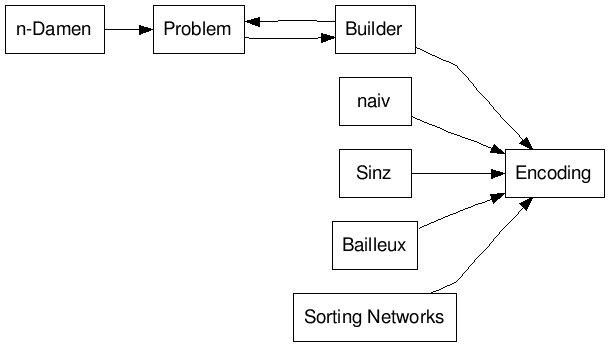
\includegraphics[width=\textwidth]{architektur.png}
\caption{Die Architektur der Implementierung}
\label{fig:architektur}
\end{figure}

In Abbildung \ref{fig:architektur} ist dargestellt, wie die grundlegende Architektur aufgebaut ist. 
Der Builder ist die Zwischenschicht zwischen den Problemen und den unterschiedlichen Kodierungen. Er erstellt das Encoding und ermöglicht dadurch den Aufruf verschiedener Kodierungen. In dieser Klasse werden die verschiedenen Constraints für $\leq$, 	$\geq$ und $\doteq$ gebaut und der Solver wird aufgerufen. Die Klasse Encoding dient als Oberklasse und ist abstrakt, damit die Signatur für die Unterklassen (Kodierungen) vorgegeben ist. 

\section{Evaluation}

\section{Schlussfolgerung und Ausblick}

%Sogar zitieren kann man \textbackslash o/ \cite[vgl.][]{invincible}.


%\begin{algorithm}
%\caption{Minimax-Suche}
%\label{alg:minimax}
%\begin{algorithmic}
%\State $\text{minimax(Spielstellung s)}$
%\State $\text{~~~~falls }spielende(s)$
%\State $\text{~~~~~~~~return }payoff(s)$
%\State $\text{~~~~} v \gets -\infty$
%\State $\text{~~~~für alle möglichen Züge }m$
%\State $\text{~~~~~~~~} f"uhreZugAus(s, m)$
%\State $\text{~~~~~~~~} v' \gets -minimax(s)$
%\State $\text{~~~~~~~~} nimmZugZur"uck(s, m)$
%\State $\text{~~~~~~~~falls }v' > v$
%\State $\text{~~~~~~~~~~~~}v \gets v'$
%\State $\text{~~~~return } v$
%\end{algorithmic}
%\end{algorithm}

%\begin{table}
%\centering
%\small %macht die Schrift kleiner
%\setlength{\tabcolsep}{.11cm} %macht den seitlichen Rand der Zellen kleiner (und damit die Tabelle schmaler)
%\begin{tabular}{|c||c|c|c|C{1.3cm}|c||c|}
%\hline
% & Base & Setup & Heuristics & Chance Pruning & Extensions & Gesamt \\ \hline \hline
%Base & - & $20$ & $22$ & $16,5$ & $18,5$ & $77$\\ \hline
%Setup & $30$ & - & $23,5$ & $19,5$ & $23$ & $96$\\ \hline
%Heuristics & $28$ & $26,5$ & - & $19,5$ & $23,5$ & $97,5$ \\ \hline
%ChancePruning & $33,5$ & $30,5$ & $30,5$ & - & $27$ & $121,5$\\ \hline
%Extensions & $31,5$ & $27$ & $26,5$ & $23$ & - & $108$ \\ \hline
%\end{tabular}
%\caption{Paarweise Ergebnisse des Turniers}
%\label{tab:roundrobin}
%\end{table}

	\clearpage
	\appendix
	\section{Literaturverzeichnis}
		% Latex-Magie von http://tex.stackexchange.com/questions/22645/hiding-the-title-of-the-bibliography
		\begingroup
			\renewcommand{\section}[2]{}
			\bibliographystyle{natdin}
			\bibliography{referenzen}
		\endgroup
\clearpage
	\section{Abbildungsverzeichnis}
		\begingroup
			\renewcommand{\section}[2]{}
			\listoffigures
		\endgroup
	\section{Tabellenverzeichnis}
		\begingroup
			\renewcommand{\section}[2]{}
			\listoftables
		\endgroup
\end{document}
